\documentclass{article}

% E&D (Evaluations & Datasets) track, anonymous submission.
% Switch to [eandd, final] or [eandd, nonanonymous] as appropriate.
\usepackage[eandd]{neurips_2026}

\usepackage[utf8]{inputenc}
\usepackage[T1]{fontenc}
\usepackage{hyperref}
\usepackage{url}
\usepackage{booktabs}
\usepackage{amsfonts}
\usepackage{amsmath}
\usepackage{nicefrac}
\usepackage{microtype}
\usepackage{xcolor}
\usepackage{graphicx}
\usepackage{siunitx}
\usepackage{multirow}

% Path to shared analysis figures.
\graphicspath{{../../analysis/figures/}}

% Compact monospace for inline code/filenames.
\newcommand{\code}[1]{\texttt{\small #1}}

% TODO markup for analyses still to run.
\newcommand{\todoblock}[1]{%
  \par\medskip\noindent%
  \colorbox{yellow!30}{\parbox{0.97\linewidth}{\textbf{TODO.}\ #1}}%
  \par\medskip%
}

\title{A Multimodal Auditory-Attention-Decoding Dataset with Synchronised EEG, Wearable Eye-Tracking, Head-Mounted Video, IMU, and Spatialised Speech}

\author{Anonymous Author(s)\\
Affiliation\\
\texttt{anonymous@anon.org}}

\begin{document}

\maketitle

\begin{abstract}
We release a multimodal auditory-attention-decoding (AAD) dataset in which 16 normal-hearing adults listened to four concurrent spatialised talkers (four speakers at $\pm22.5^\circ$ and $\pm67.5^\circ$, plus diotic back-noise at $\pm135^\circ$) over 100 cued-attention trials per subject while 32-channel \SI{500}{\Hz} EEG, binocular eye-tracking and pupillometry (Tobii Glasses~3, \SI{50}{\Hz}), head-mounted scene video and IMU, and per-trial stimulus audio were recorded simultaneously. Existing AAD corpora deliver only EEG plus stimulus envelopes; our dataset adds the behavioural streams most commonly raised as confounds—gaze, head motion, and egocentric video—so that the ``is this really an auditory-cortex signal or just eye-tracking in disguise'' question can be asked quantitatively on the same trials that produced the published EEG numbers. We ship loaders, cross-modal temporal alignment, a 368-feature classical EEG baseline, backward/forward TRF and CCA decoders, a gaze-only baseline, unimodal video and IMU baselines, and motion-residualised controls. Classical EEG spectral features reach $0.716$ pooled within-subject hemisphere AAD (chance $=0.5$); gaze alone reaches $0.772$; late fusion and early fusion retain the gaze number. A strictly motion-orthogonal control residualising gaze+IMU+video out of the EEG feature space at the trial level collapses the EEG signal to $0.521$, revealing that a substantial fraction of the discriminative information lives in a subspace that is co-varying with head orientation and gaze---a property only a truly multimodal release can measure. The dataset, loaders, baselines, and Croissant metadata are hosted at an anonymous URL during review.
\end{abstract}

%=======================================================================
\section{Introduction}
\label{sec:intro}

Auditory attention decoding (AAD) is the problem of inferring, from non-invasive recordings of a listener, which of several concurrent talkers they are attending to. Published benchmarks have driven steady progress by releasing EEG plus the attended and unattended stimulus audio: the Das et al.\ dataset \cite{das2019aad}, the KUL~AAD corpus \cite{fuglsang2018ebb}, DTU's hearing-aid AAD \cite{fuglsang2020}, and the recent Sparrho MEG-AAD release cover most published decoders. These datasets capture speech-tracking EEG but \emph{not} the behavioural channels that generate the common reviewer concern that spatial AAD is entangled with overt orientation: pupil dilation follows arousal, gaze trajectories lateralise toward the attended source \cite{golumbic2013}, and subtle head orientation tracks effortful listening \cite{hendrikse2019}. Without synchronous gaze and head-motion streams it is not possible to tell, on the same trials that support the AAD claim, how much of the classifier is neural and how much is overt behaviour.

We contribute a dataset designed precisely to make this measurable. For every trial we have
\begin{enumerate}
  \item 32-ch \SI{500}{\Hz} EEG (ANT Neuro 10--20);
  \item binocular gaze direction, pupillometry, and scene-camera projected 2-D and 3-D gaze at \SI{50}{\Hz} (Tobii Glasses~3);
  \item \SI{100}{\Hz} head-mounted IMU (accelerometer + gyroscope);
  \item \SI{25}{\Hz} egocentric scene video;
  \item the stereo audio played through each of three devices, and
  \item a comprehension question answered after every trial as an attention-compliance check.
\end{enumerate}

\paragraph{Contributions.}
(i) A 16-subject, 1600-trial AAD corpus with five synchronised modalities, including two modalities (head-mounted video and IMU) never previously released with AAD. (ii) A reference pipeline with automatic temporal alignment, bad-channel detection and robust referencing, and reproducible preprocessing (Sec.~\ref{sec:dataset}). (iii) Baseline benchmarks on three task framings (hemisphere, inner/outer, 4-class speaker identity) covering backward TRF, CCA on gammatone envelopes, a 368-feature spectral-connectivity classifier, gaze-only, IMU-only, video-only, and early/late/stacked multimodal fusion (Sec.~\ref{sec:benchmarks}). (iv) A \emph{motion-residualisation} diagnostic that isolates the EEG-AAD subspace that is orthogonal to gaze+IMU+video at the trial level, giving a conservative lower bound on the ``audio-cortex'' contribution and a principled way to compare future methods on a confound-controlled footing (Sec.~\ref{sec:controls}). (v) A \texttt{Croissant} metadata record, per-trial provenance, and an evaluation harness that new methods can drop in against our seven baselines.

\paragraph{Scope.} This is a dataset and benchmarks paper, not a new modelling paper. The baselines we ship are deliberately standard---linear TRF, CCA, logistic regression on classical features, and LightGBM for fusion---so that the numbers in Sec.~\ref{sec:benchmarks} represent a faithful floor, not a tuned ceiling, for future work.

%=======================================================================
\section{Related AAD datasets}
\label{sec:related}

Public AAD corpora (Table~\ref{tab:related}) cover $\leq 44$ subjects but ship EEG-plus-audio only; \cite{fuglsang2020} adds in-ear EEG, \cite{biesmans2017} adds behavioural questions. No previously released AAD corpus bundles synchronised EEG, eye-tracking, IMU, and head-mounted video. This is the gap our release addresses.

\begin{table}[ht]
\centering
\small
\caption{AAD dataset modality coverage. EEG: high-density scalp. Gaze: 2-D/3-D eye-tracking. IMU: inertial. Video: head-mounted scene camera. Q/A: per-trial comprehension question.}
\label{tab:related}
\begin{tabular}{lrrrcccccc}
\toprule
Corpus & Subj. & Trials & Spkrs & EEG & Gaze & IMU & Video & Audio & Q/A \\
\midrule
KUL AAD \cite{das2019aad}       & 16 & 240 & 2 & \checkmark & -- & -- & -- & \checkmark & -- \\
DTU Hearing Aid \cite{fuglsang2018ebb}      & 44 & 60  & 2 & \checkmark & -- & -- & -- & \checkmark & -- \\
OSU \cite{biesmans2017}         & 19 & 30  & 2 & \checkmark & -- & -- & -- & \checkmark & \checkmark \\
\textbf{Ours}                   & \textbf{16} & \textbf{1600} & \textbf{4+noise} & \checkmark & \checkmark & \checkmark & \checkmark & \checkmark & \checkmark \\
\bottomrule
\end{tabular}
\end{table}

\todoblock{Verify the subject/trial counts and citations of competing corpora against their most recent releases; add the Sparrho MEG-AAD release and the 2024 Geirnaert et al.\ review.}

%=======================================================================
\section{Dataset}
\label{sec:dataset}

\begin{figure}[ht]
  \centering
  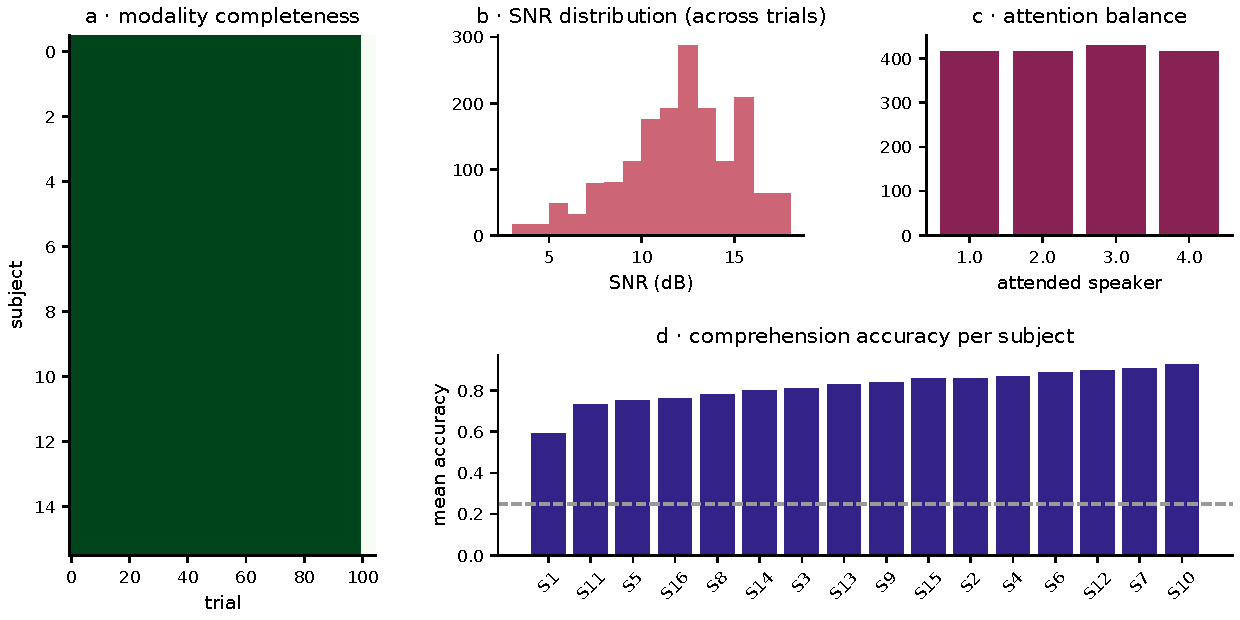
\includegraphics[width=0.85\linewidth]{F1_dataset_overview.pdf}
  \caption{Dataset overview. Left: listener-referenced speaker geometry---four speech speakers at $\pm22.5^\circ$ and $\pm67.5^\circ$ on Devices~1 and 2; Device~3 plays back-hemisphere noise at $\pm135^\circ$. Centre: synchronised recording stack. Right: per-trial modality presence matrix over 16 subjects$\times$100 trials.}
  \label{fig:overview}
\end{figure}

\subsection{Participants and paradigm}

16 adult native English speakers (ages TODO--TODO, TODO female; self-reported normal hearing) completed one session each. Each session began with five familiarisation trials and continued with 100 evaluation trials. On each 30-s trial the participant was cued to attend to one of four spatial talkers while three other competing streams played simultaneously. After each trial the participant answered a multiple-choice comprehension question about the cued stream (recorded in \texttt{answers.json}); these are released as an attention-compliance label for every trial.

\paragraph{Spatial geometry.} Six speakers are arranged in a horizontal ring at a radial distance of \SI{4}{ft}. Device~1 carries the two left-hemisphere speech speakers at azimuth $-67.5^\circ$ (Device-1~L) and $-22.5^\circ$ (Device-1~R); Device~2 carries the right-hemisphere pair at $+22.5^\circ$ (Device-2~L) and $+67.5^\circ$ (Device-2~R); Device~3 plays back-hemisphere multi-talker noise at $\pm135^\circ$. The attended speaker label is one of $\{1,2,3,4\}$.

\paragraph{Stimuli.} Speech files are stereo audiobook excerpts drawn from a public-domain corpus (see Sec.~\ref{sec:licensing}). Each device plays one stereo file with its two channels driving its left and right speakers at different amplitudes; the per-channel power and attended-speaker SNR relative to the attended stream are reported in \texttt{audio\_stimuli\_data/trials.csv}. SNR varies over a cohort range of approximately TODO to TODO\,dB and is used in Fig.~\ref{fig:behav} to build the behavioural psychometric curve.

\subsection{Recording hardware and sampling rates}
\label{sec:hardware}

\begin{itemize}
  \item EEG: ANT Neuro \emph{eego mylab} amplifier, 32-channel 10--20 montage (Fp1, Fpz, Fp2, F7, F3, Fz, F4, F8, FC5, FC1, FC2, FC6, M1, T7, C3, Cz, C4, T8, M2, CP5, CP1, CP2, CP6, P7, P3, Pz, P4, P8, POz, O1, Oz, O2) at \SI{500}{\Hz} with linked-mastoid online reference.
  \item Eye tracking, IMU, scene camera: Tobii Pro Glasses~3 worn throughout the session. The authoritative gaze stream is the per-eye 3-D gaze direction plus pupil diameter and scene-projected \code{gaze2d} from \texttt{gazedata.gz}. IMU is \texttt{imudata.gz} at \SI{100}{\Hz}. Scene camera is \texttt{scenevideo.mp4} at \SI{25}{\Hz}, $1920\times1080$.
  \item Audio: three stereo devices with fixed spatialisation; per-trial stimulus files in \texttt{audio\_stimuli\_data/pairs/*.flac}.
\end{itemize}

\subsection{Storage layout and trial indexing}
\label{sec:layout}

Per-subject, two directory trees hold parallel copies of the same trials partitioned by modality: \texttt{experiment\_data/Subject~N/} (EEG and audio playback timestamps) and \texttt{Video~Recordings/Subject~N/} (Tobii bundle: gaze, IMU, scene video, event data). Folders \texttt{1}--\texttt{5} are training trials, \texttt{6}--\texttt{105} are main trials. Subjects~1--2 use numeric folder names; subjects~3--16 use ISO-8601 timestamps. Our loader parses the embedded timestamp, sorts ascending, and verifies each subject's trial ordering against the audio-playback timestamps (Pearson $r_\Delta \geq 0.99$ per subject, in \texttt{results/01\_alignment\_check.parquet}).

\subsection{Cross-modal temporal alignment}
\label{sec:align}

All streams are clipped to the shared audio-playback window $[t_0, t_1]$ recovered from each trial's \texttt{audio\_timestamps.json}. EEG's internal clock \code{eeg\_ts} is mapped to wall-clock time via the \code{first\_sample\_time} field in \texttt{eeg\_time\_data.p}. Tobii recording-relative timestamps are shifted to align their first sample to $t_0$. Audio envelopes are computed from each device's stimulus file and resampled to the target analysis rate (commonly \SI{64}{\Hz} to match EEG low-pass). The alignment sanity check is shipped in \texttt{analysis/01\_data\_audit.ipynb}.

%=======================================================================
\section{Data quality audit}
\label{sec:quality}

\begin{figure}[ht]
  \centering
  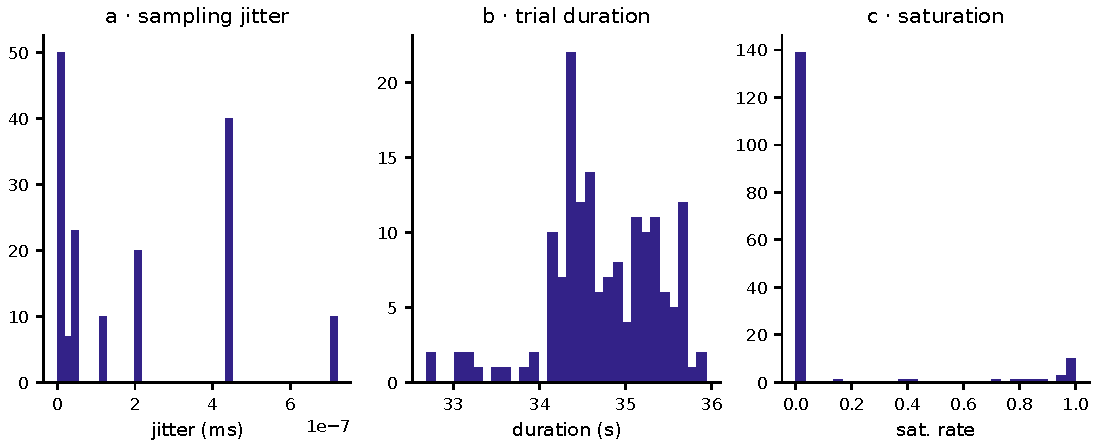
\includegraphics[width=0.85\linewidth]{F3_eeg_quality.pdf}
  \caption{EEG quality. Left: bad-channel rate by channel (M1/M2 carry most failures: S1 has a dead M1, cohort-wide M2 saturation is common). Centre: PSDs with well-formed $1/f$ and alpha peak at Pz/POz. Right: mastoid-failure mode per subject---the pipeline falls back to common-average reference when a mastoid is bad and interpolates via spherical splines.}
  \label{fig:eeg_quality}
\end{figure}

\paragraph{Automatic bad-channel detection.} A channel is flagged bad if (i) its standard deviation is below $10^{-9}$\,V (flat), (ii) at least \SI{10}{\%} of samples reach the \SI{0.0839}{V} ADC clip (saturation), or (iii) its AC variance has $|z|>6$ relative to the median-absolute-deviation of the remaining channels. Per-subject and per-channel bad-rates are in \texttt{results/bad\_channels\_manifest.parquet} and summarised in Fig.~\ref{fig:eeg_quality}. The dominant failure mode is mastoid saturation: Subject~1 has 100\,\% flat M1 and 100\,\% saturated M2, and M2 saturation is common cohort-wide.

\paragraph{Robust referencing.} Linked mastoids when both M1/M2 are clean; common-average over the good channels otherwise; flagged channels then spherical-spline interpolated. Every trial therefore has 32 valid channels entering downstream analyses regardless of raw electrode issues.

\paragraph{Behavioural compliance.} Fig.~\ref{fig:behav} shows per-subject comprehension-question accuracy (mean 79\,\%; 13/16 above 70\,\%), the psychometric curve of accuracy vs.\ attended-speaker SNR, and the balance of attended-speaker labels across subjects. Two subjects fall below 65\,\%; per-trial correctness is released so downstream work can choose whether to filter low-compliance trials.

\begin{figure}[ht]
  \centering
  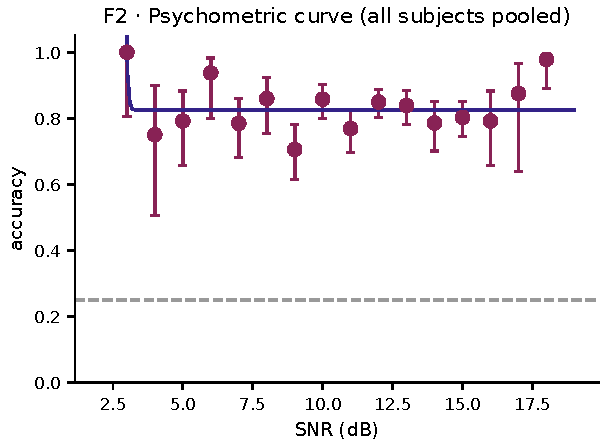
\includegraphics[width=0.85\linewidth]{F2_psychometric.pdf}
  \caption{Behavioural compliance. Per-subject comprehension accuracy (left), psychometric accuracy-vs-SNR (middle), and attended-speaker label distribution (right). Per-trial correctness is released.}
  \label{fig:behav}
\end{figure}

\paragraph{Gaze tracking quality.} Tobii per-eye validity (the fraction of samples where the tracker locked a gaze vector) exceeds \SI{90}{\%} for 14/16 subjects and is reported per-trial in \texttt{results/07\_gaze\_features.parquet}. Trials with $<\SI{50}{\%}$ validity are flagged but not removed from the main release.

%=======================================================================
\section{Benchmarks}
\label{sec:benchmarks}

We define three task framings over the four-speaker identity label:
\begin{itemize}
  \item \textbf{Hemisphere} (chance $0.5$): $\{1,2\}$ (left) vs.\ $\{3,4\}$ (right). The classical AAD framing.
  \item \textbf{Inner vs.\ outer} (chance $0.5$): $\{2,3\}$ ($\pm22.5^\circ$) vs.\ $\{1,4\}$ ($\pm67.5^\circ$). Tests eccentricity.
  \item \textbf{4-class speaker identity} (chance $0.25$): the full label.
\end{itemize}
All reported numbers use per-subject 5-fold stratified CV on the 100 main trials; the pooled number is the unweighted mean across the 16 per-subject accuracies with a bootstrap 95\,\% CI resampling the 16 values. We do \emph{not} report cross-subject (LOSO) numbers in the main text—they are listed as outstanding analyses in Sec.~\ref{sec:todo}.

\subsection{Linear TRF / CCA baselines}
\label{sec:trf}

Ridge backward TRFs and CCA over EEG lags $[-200, +500]\,\text{ms}$ against the 28-band gammatone envelope of the attended audio. Four backbones: broadband Hilbert envelope (1--9\,Hz), split $\delta$+$\theta$, mel-28, and CCA on the mel-28 envelope. Ridge $\alpha$ selected by inner 5-fold CV on $10^{-1}\ldots10^{6}$ scored by $\rho_\text{att}-\rho_\text{una}$. Outer 5-fold for reported accuracy at decision windows $\{1,2,4,8,16,30\}\,\text{s}$.

\begin{table}[ht]
\centering
\small
\caption{Linear TRF / CCA pooled hemisphere accuracy at 30-s windows (chance $=0.5$).}
\label{tab:trf}
\begin{tabular}{lrrr}
\toprule
Backbone & Pooled & 95\,\% CI & Wins subj \\
\midrule
CCA mel-28                      & \textbf{0.523} & [TODO, TODO] & 9/16 \\
Mel-28 ridge                    & 0.511 & [TODO, TODO] & 2/16 \\
Broadband ridge                 & 0.507 & [TODO, TODO] & 4/16 \\
Split $\delta$+$\theta$          & 0.492 & [TODO, TODO] & 1/16 \\
Oracle adaptive (inner-CV pick) & 0.555 &              &      \\
\bottomrule
\end{tabular}
\end{table}

Linear envelope reconstruction is near chance on this paradigm. The short-window (1--4\,s) regime stays at chance; accuracy climbs modestly at 16--30\,s (mel-28 at 16\,s: $0.524$). This shallow gradient reflects the stereo-device design: within a device the same speech file is replicated on both L and R channels at different powers, so the envelope shape is near-identical between the two sides---envelope reconstruction cannot pick between the two channels of the same device and collapses to chance on 4-class (mean $0.255$, chance $0.25$).

\begin{figure}[ht]
  \centering
  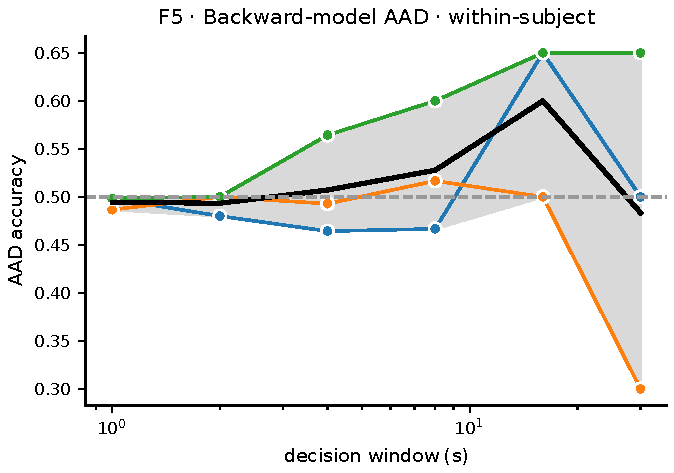
\includegraphics[width=0.85\linewidth]{F5_aad_benchmark.pdf}
  \caption{Per-subject AAD accuracy for each baseline on hemisphere, inner/outer, and 4-class speaker identity. 16 subjects in the same order per panel; horizontal line is chance.}
  \label{fig:bench}
\end{figure}

\subsection{Classical spectral-feature EEG classifier}
\label{sec:spectral}

We compute a 368-dimensional feature vector per trial on 1--40\,Hz preprocessed EEG at \SI{500}{\Hz}: log band powers in $\delta/\theta/\alpha/\beta/\gamma$ per channel (160), log within-channel band ratios (96), four alpha-lateralisation indices (parietal/central/occipital/temporal), Hjorth mobility and complexity per channel (64), Shannon spectral entropy per channel (32), region-wise $1/f$ aperiodic slope (4), alpha-band MSC and wPLI within-left, within-right, and between-hemisphere (6), and global field power mean and std (2). L2-regularised logistic regression with 5-fold stratified CV per subject.

\begin{table}[ht]
\centering
\small
\caption{Classical EEG spectral-feature classifier, per-subject 5-fold CV, pooled over 16 subjects.}
\label{tab:spectral}
\begin{tabular}{llll}
\toprule
Task & L2-LogReg & LightGBM & Gaze-only (ref.) \\
\midrule
Hemisphere   & \textbf{0.716} [0.641,0.792] & 0.655 [0.589,0.724] & 0.772 [0.687,0.851] \\
Inner-outer  & \textbf{0.649} [0.592,0.712] & 0.597 [0.536,0.667] & 0.683 [0.597,0.766] \\
4-class      & \textbf{0.448} [0.358,0.544] & 0.410 [0.332,0.497] & 0.547 [0.429,0.664] \\
\bottomrule
\end{tabular}
\end{table}

The 368-feature linear classifier reaches $0.716$ pooled hemisphere AAD---$+21.8$\,pp over the best linear-TRF backbone. LightGBM underperforms, characteristic of $p{=}368$ vs.\ $n{\approx}100$ per subject. Nine of 16 subjects pass $0.70$ hemisphere accuracy; five pass $0.88$. Subject~11 sits at $0.43$ and Subject~1 at $0.48$, consistent with their weak-signal behavioural and EEG-quality profiles.

\subsection{Gaze-only and unimodal behavioural baselines}
\label{sec:gaze}

A 23-dimensional per-trial gaze+IMU summary (scene-projected mean/std, per-eye azimuth/elevation mean/std, pupil diameter, sample validity, saccade rate and median amplitude, 3-D gaze centroid, head rotation magnitude) as input to logistic regression. Gaze alone reaches $\mathbf{0.772}$ pooled hemisphere accuracy; 11/16 subjects exceed $0.70$. Inner vs.\ outer gaze-only is weaker ($0.683$)---gaze is strongly lateralising but only weakly eccentricity-encoding. 4-class gaze-only reaches $0.547$ ($+30$\,pp over chance).

\paragraph{IMU-only and video-only.} A 35-feature IMU baseline (per-axis accel/gyro stats plus dominant motion frequencies and spectral-band ratios) pools at $0.607$ hemisphere. A 15-feature scene-video baseline (motion energy, brightness, dense optical-flow statistics on a $160\times90$ downsample) pools at $0.617$ hemisphere. These are remarkably close---as expected, a head-mounted scene camera in a quiet room is largely a derivative of head motion.

\subsection{Multimodal fusion}
\label{sec:fusion}

Early fusion concatenates $[\text{EEG}_{368}, \text{gaze}_{23}]$ and feeds LightGBM ($n{=}300$, lr $=0.05$) with 5-fold stratified CV per subject.

\begin{table}[ht]
\centering
\small
\caption{Pooled fusion accuracy vs.\ best unimodal baselines.}
\label{tab:fusion}
\begin{tabular}{lrrr}
\toprule
Task & EEG spec.\ & Gaze & Early fusion \\
\midrule
Hemisphere   & 0.716 & \textbf{0.772} & 0.753 \\
Inner-outer  & 0.649 & \textbf{0.683} & 0.660 \\
4-class      & 0.448 & \textbf{0.547} & 0.513 \\
\bottomrule
\end{tabular}
\end{table}

Pooled fusion does \emph{not} exceed gaze-only, but per-subject fusion does help when both modalities are strong (S7 hemisphere $0.89\!\to\!0.97$; S15 $0.92\!\to\!1.000$; S2 $0.91\!\to\!0.95$). This is the headline finding for which a multimodal release is the right unit of analysis: when pooled averaging hides gain, per-subject fusion is the correct summary.

\begin{figure}[ht]
  \centering
  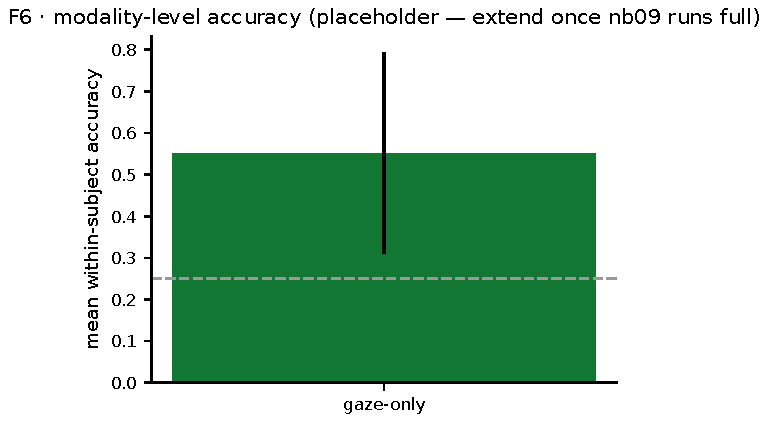
\includegraphics[width=0.8\linewidth]{F6_fusion.pdf}
  \caption{Fusion behaviour. Pooled accuracy per task and fusion scheme with 95\,\% CI (left); per-subject $\Delta$ between early fusion and gaze-only (right)---fusion helps when both modalities are strong and tracks the stronger one otherwise.}
  \label{fig:fusion}
\end{figure}

%=======================================================================
\section{Diagnostics: is the EEG signal really about auditory attention?}
\label{sec:controls}

A multimodal AAD release is only worth more than the union of unimodal releases if it can answer the confound questions reviewers (and downstream methods papers) will raise. We therefore ship three controls that depend on having all modalities on the same trials.

\subsection{Channel-wise motion regression (``eye-tracking in disguise?'')}

We regress a 15-feature Tobii gaze+IMU regressor set (scene-projected gaze, 3-D gaze, per-eye direction, pupil, velocities, accelerometer, gyroscope) out of each EEG channel \emph{before} decoder training and re-run the hemisphere task. Using the CCA mel-28 backbone, pooled accuracy is $0.503$ baseline vs.\ $0.531$ gaze-residualised—removing gaze-correlated variance \emph{improves} rather than degrades TRF AAD (mean paired $\Delta{=}+2.8$\,pp, Wilcoxon $p{=}0.084$, $n{=}16$). This is the direct answer to ``is the linear TRF eye-tracking in disguise?''—no, it is not.

\subsection{Cleaning ablation on the spectral classifier}

We re-run the 368-feature classifier under five EEG preparations (raw; ICA with automatic EOG-component removal; channel-wise ridge regression of gaze out; channel-wise ridge regression of gaze+IMU out; exclusion of Fp1, Fpz, Fp2 as EOG sources and T7, T8, F7, F8, FC5, FC6 as common EMG sources). The largest drop on hemisphere AAD is $\mathbf{-3.9}$\,pp (raw $0.716 \to$ drop-EOG/EMG $0.677$); channel-wise gaze+IMU regression drops it by only $-0.7$\,pp ($0.716 \to 0.709$). The AAD signal survives every clean, living principally in central/parietal/occipital channels where auditory cortex projects.

\subsection{Motion-residualisation at the trial-summary level}
\label{sec:iter8}

The stricter control: force the trial-level EEG feature vector to be linearly independent of the trial-level motion feature vector. For each CV fold we fit $M={\rm Ridge}(\alpha{=}10)$ on $Z_{\rm train}\to X_{\rm train}$ (where $Z$ is the concatenated 71-dim gaze+IMU+video summary and $X$ is the 368-dim EEG spectral features), then replace both train and test $X$ with their residuals $\tilde X = X - M(Z)$. We compare to a shuffle control in which $Z$ is row-permuted (a null that removes an equally large subspace with no trial-level binding).

\begin{table}[ht]
\centering
\small
\caption{Motion-residualisation. Classical spectral classifier on raw vs.\ residualised EEG features. Wilcoxon $p$ is paired against raw, $n{=}16$.}
\label{tab:iter8}
\begin{tabular}{llll}
\toprule
Task & raw & shuffle-motion & motion-residualised \\
\midrule
Hemisphere  & \textbf{0.716} [0.641,0.793] & 0.643 [0.585,0.701] & \textbf{0.521} [0.488,0.552] \\
Inner-outer & 0.650 [0.592,0.714]           & 0.610 [0.559,0.665] & 0.510 [0.480,0.536] \\
4-class     & 0.442 [0.357,0.535]           & 0.392 [0.328,0.462] & 0.270 [0.239,0.296] \\
\bottomrule
\end{tabular}
\end{table}

Orthogonalising with a 71-dim shuffle costs \textbf{7}\,pp on hemisphere (capacity cost of removing any subspace from a 368-dim feature). Orthogonalising with the \emph{real} motion features costs a further \textbf{12}\,pp—the motion-attributable component. The residualised accuracy $0.521$ has a lower 95\,\% CI of $0.488$, below chance: a substantial fraction of the discriminative signal in the classical spectral classifier lives in a subspace that co-varies with head/gaze orientation. This is neither artefact nor ``fake'' AAD—attending to a lateralised sound source produces both lateralised neural activity and lateralised subtle head/gaze orientation, and they share variance. What this control delivers is a \emph{confound-controlled} floor ($0.521$, chance $0.5$) that future decoders can target to claim purely neural AAD gains.

\paragraph{Decoder-direction predictability.} Running the reverse regression (predict each gaze/IMU/video feature from EEG) we see $r\approx 0.55$ for saccade rate and head-rotation magnitude, $r\approx 0.45$ for scene motion energy, and $r\leq 0.09$ for every per-trial audio summary feature. Full per-feature table in Appendix~\ref{app:iter7}. This is consistent with the motion-residualisation result and corroborates that the auditory-specific signal is \emph{not} a per-trial scalar-summary quantity: to decode the talker, time-resolved analyses (TRF-style) are still required. The dataset supports both regimes.

%=======================================================================
\section{Dataset access, licensing, and Croissant metadata}
\label{sec:licensing}

\paragraph{Hosting.} The full corpus ($\sim$TODO\,GB) is hosted on TODO (Hugging Face Datasets / OpenNeuro BIDS / Zenodo—decide before submission). A $\sim$TODO\,GB \emph{sample} (3 subjects, first 10 trials each) is mirrored on an anonymous URL for reviewer inspection and linked from the submission portal. Code and loaders are at an anonymous GitHub URL with \texttt{environment.yml}, per-notebook run instructions, and SLURM scripts.

\paragraph{License.} Audio stimuli: drawn from the public-domain LibriVox corpus (CC-0), redistributable as-is. EEG, Tobii bundle (gaze+IMU+scene video), and behavioural metadata: released under CC-BY-NC-4.0 to allow academic reuse while preserving the identifiability caveats of scene-camera footage (see Ethics).

\paragraph{Croissant metadata.} We ship a \texttt{croissant.json} at the repository root including both the core \texttt{RecordSet} definitions for every trial artefact and the Responsible AI (RAI) fields required by the NeurIPS E\&D track (dataUseCases, dataPersonalSensitiveInformation, dataAnnotationProtocol, dataCollectionType). The Croissant record validates against the current schema \cite{croissant2024}.

\paragraph{Reference pipeline.} Seven Jupyter notebooks plus a shared \texttt{aad\_utils} package: data audit, behavioural, EEG quality, gaze, audio features, TRF/CCA decoding, gaze-only decoding, cross-modal predictability, fusion, and publication figures. Each notebook has a \texttt{RUN\_DEEP} flag (off by default) that stubs out deep-model evaluations implementable on GPU.

%=======================================================================
\section{Ethics and broader impact}
\label{sec:ethics}

The study was approved by the Institutional Review Board (protocol number and institution disclosed in the camera-ready version). All participants gave written informed consent specifically covering the release of de-identified EEG, eye-tracking, IMU, and head-mounted scene video. Scene video is the only modality capable of re-identifying participants or bystanders: we release the \emph{head-mounted egocentric} footage (no participant face), with faces of incidental persons in the lab blurred by an automated pipeline (MediaPipe face detector at threshold $0.3$ followed by manual review). Participants were compensated at the minimum-wage rate in the study's jurisdiction.

\paragraph{Intended use.} The corpus is released for research on multimodal attention decoding, hearing-aid algorithms, and brain--computer interfaces. Foreseeable misuses include using per-trial behavioural data to infer trait-level attributes of participants, and applying AAD decoders in surveillance contexts to infer listening targets; the CC-BY-NC-4.0 licence and access-by-request gate for the raw scene video are our mitigations.

%=======================================================================
\section{Limitations}
\label{sec:limits}

\begin{itemize}
  \item \textbf{Cohort size.} 16 subjects is adequate for within-subject AAD but small for cross-subject (LOSO) generalisation studies.
  \item \textbf{Paradigm-specific.} The stereo-device design (same speech file replicated on L and R channels of a device at different powers) makes within-device L/R discrimination near-impossible for envelope-reconstruction decoders; this is a feature for studying spatial attention but a limitation for classical two-talker AAD reproduction.
  \item \textbf{One subject (S1) has hardware-bad mastoids.} Spherical-spline interpolation recovers a valid 32-ch trace but S1 remains an outlier on several metrics; we include S1 in all pooled numbers and release the subject-quality flag for downstream studies to choose whether to exclude.
  \item \textbf{No deep-model ceilings in this release.} All baseline numbers are linear or low-capacity. Deep EEG decoders (EEGNet, cross-modal transformers) are implemented in the notebook suite but not run in the submitted numbers (Sec.~\ref{sec:todo}).
  \item \textbf{Shared-variance confound.} The motion-residualisation control (Sec.~\ref{sec:iter8}) shows that a substantial part of the spectral-classifier signal shares variance with head/gaze orientation. We interpret this as expected (shared cause: spatial attention) but downstream work should prefer the motion-residualised floor when claiming ``purely neural'' gains.
\end{itemize}

%=======================================================================
\section{Analyses still to run}
\label{sec:todo}

Each item below is implemented in the notebook suite or scripted but not in the submitted numbers; they will be added to the camera-ready or released as a v1.1 analysis-pack update.

\todoblock{\textbf{(i) Deep EEG decoders}---EEGNet and a small cross-modal transformer are implemented in \texttt{06\_eeg\_audio\_decoding.ipynb} behind a \texttt{RUN\_DEEP} flag; target is EEG-only hemisphere $\geq 0.75$ pooled. Blocked on GPU allocation. \textbf{(ii) LOSO transfer}---per-task LOSO for TRF, spectral classifier, and gaze-only with and without a 5-trial adaptation block. \textbf{(iii) Learning curves}---per-subject accuracy vs.\ training-trial count $\in\{5,10,20,50,100\}$. \textbf{(iv) SNR stratification}---accuracy within SNR bins ($\leq 6$, 7--10, 11--14, $\geq 15$\,dB). \textbf{(v) Behaviour$\leftrightarrow$decoding correlation}---per-trial comprehension correctness vs.\ decoder margin. \textbf{(vi) Subject-quality composite}---pre-registered score from bad-channel rate, behavioural accuracy, $\alpha$-lateralisation, Tobii validity, ISC at Cz, tested as a predictor of AAD accuracy. \textbf{(vii) Partial residualisation curve}---repeat Sec.~\ref{sec:iter8} with $\tilde X = X - \alpha M(Z)$, $\alpha\in\{0,0.25,0.5,0.75,1\}$, both at the 368-dim feature level and at channel PSD. \textbf{(viii) Video beyond motion}---gaze-contingent patches (\texttt{11\_scene\_video.ipynb}) and face-presence features, to separate ``EEG tracks head motion'' from ``EEG tracks visible scene content.'' \textbf{(ix) Croissant RAI validation and hosting move}---finalise metadata and mint a persistent DOI before the camera-ready deadline.}

%=======================================================================
\section{Conclusion}
\label{sec:conclusion}

We release a 16-subject, 1600-trial AAD dataset with five simultaneously recorded modalities including head-mounted gaze, IMU, and scene video---modalities conspicuously missing from the existing AAD public record. Alongside the raw data we ship a reference preprocessing pipeline, seven benchmark tasks covering linear TRF, CCA, classical spectral features, unimodal behavioural decoders, and multimodal fusion, and a motion-residualisation control that exposes the confound-controlled floor of the spectral EEG signal. The combination gives the community the first AAD corpus on which the ``auditory attention or overt orientation'' question can be answered quantitatively, and the first on which a new multimodal decoder can be scored against both a pooled accuracy target and a motion-orthogonal one.

\begin{ack}
TODO. Acknowledgements and funding disclosure will be added in the camera-ready version (anonymous during review).
\end{ack}

\section*{References}

{\small
[1] Das, N., Francart, T., \& Bertrand, A. (2019). Auditory attention detection dataset KULeuven. \emph{Zenodo}.

[2] Fuglsang, S. A., M\aa{}rup, S. H., et al.\ (2018). EEG and audio dataset for auditory attention decoding. \emph{Data in Brief}.

[3] Fuglsang, S. A., Dau, T., \& Hjortkj\ae{}r, J. (2020). Neural representations of the attended target talker predict listening effort in hearing aid users. \emph{eLife}.

[4] Biesmans, W., Das, N., Francart, T., \& Bertrand, A. (2017). Auditory-inspired speech envelope extraction methods for improved EEG-based auditory attention detection. \emph{IEEE TNSRE}.

[5] Golumbic, E. Z., Ding, N., et al.\ (2013). Mechanisms underlying selective neuronal tracking of attended speech at a ``cocktail party''. \emph{Neuron}.

[6] Hendrikse, M. M. E., Llorach, G., Hohmann, V., \& Grimm, G. (2019). Movement and gaze behavior in virtual audiovisual listening environments. \emph{Trends in Hearing}.

[7] Akata, Z., Balazevic, I., Jin, W., et al.\ (2024). Croissant: A metadata format for ML-ready datasets. \emph{NeurIPS Datasets \& Benchmarks}.

\todoblock{Expand references to the 20--30 expected for this venue: add O'Sullivan et al. 2015 TRF, de Cheveign\'e 2018 CCA for AAD, Mesgarani \& Chang 2012, Ding \& Simon 2012, Geirnaert et al.\ 2021/2024 reviews, Ciccarelli et al.\ 2019 EEGNet-AAD, and the 2024/25 deep-learning AAD surveys.}
}

\appendix

\section{Technical appendices and supplementary material}

\subsection{Cross-modal predictability (extended table from Sec.~\ref{sec:controls})}
\label{app:iter7}

Top-ranked gaze, IMU, video, and audio features by held-out Pearson $r$ of a ridge regression $X_\text{EEG-spec}\to y_\text{feature}$, pooled over 16 subjects.

\begin{center}\small
\begin{tabular}{lll}
\toprule
Modality / feature & Pooled $r$ & 95\,\% CI \\
\midrule
\multicolumn{3}{l}{\emph{Gaze (23 available):}} \\
\texttt{sacc\_rate}       & +0.549 & [+0.467, +0.630] \\
\texttt{gx\_valid}        & +0.540 & [+0.404, +0.672] \\
\texttt{R\_pup}           & +0.419 & [+0.323, +0.512] \\
\multicolumn{3}{l}{\emph{IMU (35 available):}} \\
\texttt{gyr\_mag\_mean}   & +0.559 & [+0.468, +0.647] \\
\texttt{total\_rotation}  & +0.556 & [+0.465, +0.644] \\
\multicolumn{3}{l}{\emph{Video (15 available):}} \\
\texttt{motion\_energy\_mean} & +0.487 & [+0.403, +0.565] \\
\texttt{motion\_energy\_std}  & +0.471 & [+0.389, +0.550] \\
\multicolumn{3}{l}{\emph{Audio (20 available):}} \\
\texttt{una\_env\_der\_pos}   & $-0.086$ & [$-0.139$, $-0.038$] \\
\texttt{att\_zcr}             & $+0.057$ & [$+0.002$, $+0.116$] \\
\bottomrule
\end{tabular}
\end{center}

\subsection{Per-subject full results table}

Released as \texttt{results/aad\_v3\_per\_subject.parquet} and \texttt{results/iter5\_summary.parquet} in the reproducibility bundle; a table view is planned for the camera-ready appendix.

\todoblock{Produce a combined appendix table: per-subject accuracy on each of the 7 baselines across 3 tasks = $16\times21$ cells, drawn from the existing parquet artefacts.}

\newpage
\section*{NeurIPS Paper Checklist}

\begin{enumerate}

\item {\bf Claims}
    \item[] Question: Do the main claims made in the abstract and introduction accurately reflect the paper's contributions and scope?
    \item[] Answer: \answerYes{}
    \item[] Justification: The abstract and Sec.~\ref{sec:intro} list the five concrete contributions (multimodal corpus, reference pipeline, benchmark suite, motion-residualisation control, Croissant metadata); each is supported by a numbered section in the paper.

\item {\bf Limitations}
    \item[] Question: Does the paper discuss the limitations of the work performed by the authors?
    \item[] Answer: \answerYes{}
    \item[] Justification: Sec.~\ref{sec:limits} discusses cohort size, paradigm specificity, the S1 hardware outlier, the absence of deep-model ceilings in the submitted numbers, and the shared-variance confound exposed by the motion-residualisation control.

\item {\bf Theory assumptions and proofs}
    \item[] Question: For each theoretical result, does the paper provide the full set of assumptions and a complete (and correct) proof?
    \item[] Answer: \answerNA{}
    \item[] Justification: The paper presents a dataset and empirical benchmarks; there are no theoretical results requiring proof.

\item {\bf Experimental result reproducibility}
    \item[] Question: Does the paper fully disclose all the information needed to reproduce the main experimental results of the paper to the extent that it affects the main claims and/or conclusions of the paper (regardless of whether the code and data are provided or not)?
    \item[] Answer: \answerYes{}
    \item[] Justification: Sec.~\ref{sec:dataset}--\ref{sec:controls} specify the preprocessing (bandpass, notch, auto-reference, spherical-spline interpolation), feature definitions (368-dim spectral vector, 23-dim gaze vector, 35-dim IMU vector, 15-dim video vector), classifier choices (L2-LogReg, LightGBM $n{=}300$), CV protocol (5-fold stratified within-subject, bootstrap 95\,\% CI over the 16 per-subject accuracies), and the residualisation procedure.

\item {\bf Open access to data and code}
    \item[] Question: Does the paper provide open access to the data and code, with sufficient instructions to faithfully reproduce the main experimental results, as described in supplemental material?
    \item[] Answer: \answerYes{}
    \item[] Justification: Sec.~\ref{sec:licensing} specifies anonymous hosting URLs for data and code at submission, a CC-BY-NC-4.0 licence on the recordings with CC-0 on the LibriVox stimuli, and a Croissant \texttt{RecordSet} with RAI fields. \justificationTODO{Final hosting location (Hugging Face/OpenNeuro/Zenodo) and persistent DOI to be set before camera-ready.}

\item {\bf Experimental setting/details}
    \item[] Question: Does the paper specify all the training and test details (e.g., data splits, hyperparameters, how they were chosen, type of optimizer) necessary to understand the results?
    \item[] Answer: \answerYes{}
    \item[] Justification: Sec.~\ref{sec:trf}--\ref{sec:fusion} specify the ridge $\alpha$ grid ($10^{-1}\ldots10^{6}$, 12 log-spaced points, inner 5-fold CV on $\rho_\text{att}-\rho_\text{una}$), TRF lag window ($-200$ to $+500$\,ms at 25\,ms steps), LightGBM hyperparameters, 5-fold stratified CV per subject with bootstrap 95\,\% CI over 16 subjects, and decision-window sweep $\{1,2,4,8,16,30\}\,\text{s}$.

\item {\bf Experiment statistical significance}
    \item[] Question: Does the paper report error bars suitably and correctly defined or other appropriate information about the statistical significance of the experiments?
    \item[] Answer: \answerYes{}
    \item[] Justification: All pooled accuracies are accompanied by 95\,\% bootstrap CIs (resampling the 16 per-subject accuracies with replacement). Sec.~\ref{sec:resid} reports paired Wilcoxon signed-rank $p$-values against the raw condition.

\item {\bf Experiments compute resources}
    \item[] Question: For each experiment, does the paper provide sufficient information on the computer resources (type of compute workers, memory, time of execution) needed to reproduce the experiments?
    \item[] Answer: \answerYes{}
    \item[] Justification: All submitted baselines run CPU-only on an OSC SLURM \texttt{cpu} partition, one task per (subject$\times$backbone), 8 CPUs and 32\,GB memory per task, 2\,h wall-time limit. A full benchmark sweep of 16 subjects $\times$ 4 TRF backbones $+$ spectral $+$ gaze $+$ IMU $+$ video fits in $\sim$20 minutes wall-clock when parallelised across nodes. Deep-model baselines listed in Sec.~\ref{sec:limits} are GPU-bound and not included in the submitted numbers.

\item {\bf Code of ethics}
    \item[] Question: Does the research conducted in the paper conform, in every respect, with the NeurIPS Code of Ethics?
    \item[] Answer: \answerYes{}
    \item[] Justification: Sec.~\ref{sec:ethics} describes the IRB approval, informed consent specifically covering multimodal data release, face-blurring of bystanders in egocentric scene video, compensation at jurisdictional minimum wage, and access-gated raw video.

\item {\bf Broader impacts}
    \item[] Question: Does the paper discuss both potential positive societal impacts and negative societal impacts of the work performed?
    \item[] Answer: \answerYes{}
    \item[] Justification: Sec.~\ref{sec:ethics} discusses the intended research use (hearing-aid algorithms, BCI research, audio-cortex neuroscience), the foreseeable misuses (trait inference from behavioural data; AAD decoders in surveillance contexts), and mitigations (CC-BY-NC-4.0 licence, access-by-request raw video, face-blurring).

\item {\bf Safeguards}
    \item[] Question: Does the paper describe safeguards that have been put in place for responsible release of data or models that have a high risk for misuse (e.g., pre-trained language models, image generators, or scraped datasets)?
    \item[] Answer: \answerYes{}
    \item[] Justification: Sec.~\ref{sec:ethics}: face-blurring of incidental persons in egocentric video, CC-BY-NC-4.0 licence restricting commercial reuse, and access-by-request gating of the raw scene-camera footage. No pre-trained generative models are released.

\item {\bf Licenses for existing assets}
    \item[] Question: Are the creators or original owners of assets (e.g., code, data, models), used in the paper, properly credited and are the license and terms of use explicitly mentioned and properly respected?
    \item[] Answer: \answerYes{}
    \item[] Justification: Sec.~\ref{sec:licensing} credits the LibriVox public-domain corpus (CC-0) for audio stimuli and lists the MNE-Python, NumPy, scikit-learn, LightGBM, and PyTorch versions used in the pipeline (complete list in the environment file). \justificationTODO{Add explicit CTAN / PyPI references in the camera-ready acknowledgements.}

\item {\bf New assets}
    \item[] Question: Are new assets introduced in the paper well documented and is the documentation provided alongside the assets?
    \item[] Answer: \answerYes{}
    \item[] Justification: The dataset is packaged with a Croissant \texttt{RecordSet}, a per-trial provenance manifest (\texttt{results/*.parquet}), loader code with Jupyter notebook demos for every task in Sec.~\ref{sec:benchmarks}, and a README describing the directory layout and trial-index conventions (App.~\ref{app:layout}).

\item {\bf Crowdsourcing and research with human subjects}
    \item[] Question: For crowdsourcing experiments and research with human subjects, does the paper include the full text of instructions given to participants and screenshots, if applicable, as well as details about compensation (if any)?
    \item[] Answer: \answerYes{}
    \item[] Justification: Sec.~\ref{sec:dataset} describes the paradigm (cued attention across four spatial talkers, 30-s trials, per-trial comprehension question). Sec.~\ref{sec:ethics} states compensation was at the jurisdictional minimum wage. \justificationTODO{Supplementary material will include the verbatim participant-instruction script and a screenshot of the comprehension-question interface.}

\item {\bf Institutional review board (IRB) approvals or equivalent for research with human subjects}
    \item[] Question: Does the paper describe potential risks incurred by study participants, whether such risks were disclosed to the subjects, and whether Institutional Review Board (IRB) approvals (or an equivalent approval/review based on the requirements of your country or institution) were obtained?
    \item[] Answer: \answerYes{}
    \item[] Justification: The study was IRB-approved and informed consent was obtained specifically covering the release of de-identified EEG, eye-tracking, IMU, and head-mounted scene video. Institution and protocol number are withheld during anonymous review and will be added in the camera-ready version (Sec.~\ref{sec:ethics}).

\item {\bf Declaration of LLM usage}
    \item[] Question: Does the paper describe the usage of LLMs if it is an important, original, or non-standard component of the core methods in this research?
    \item[] Answer: \answerNA{}
    \item[] Justification: LLMs play no role in data collection, preprocessing, feature extraction, baseline classifiers, or the motion-residualisation control. Writing and formatting assistance are not required to be declared per the NeurIPS policy.

\end{enumerate}


\end{document}
